\section{Connections}
\subsection{Overview High Level Connections}
\begin{figure}[h!]
    \centering
    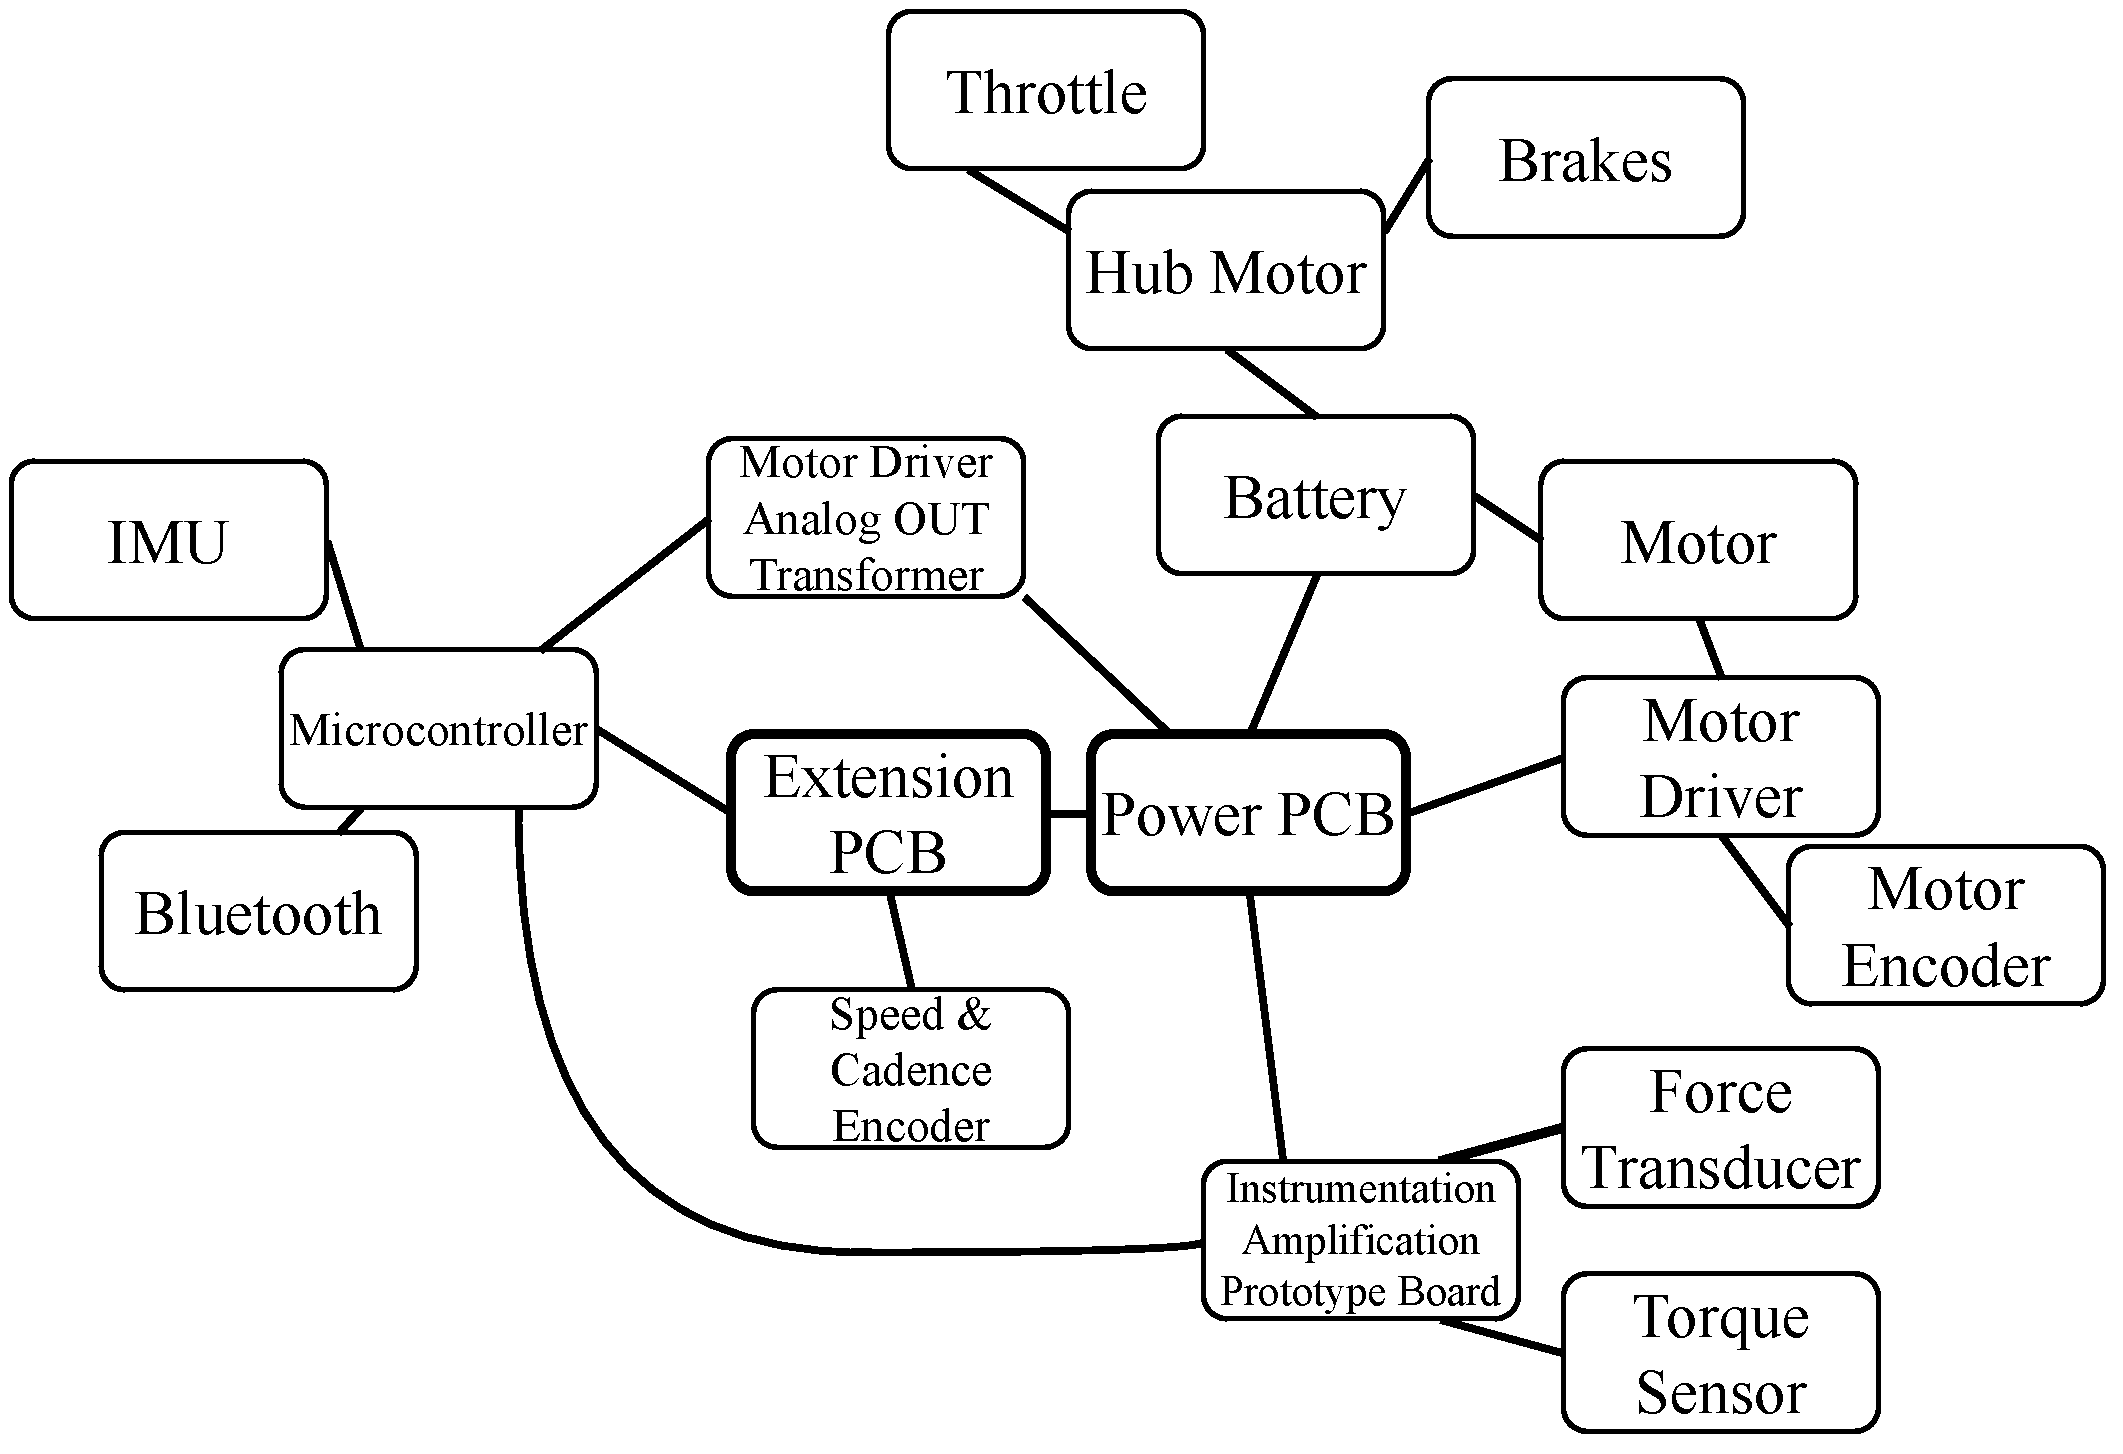
\includegraphics[width=0.96\textwidth]{Img/Overview_sbw_system.pdf}
    \caption{Web of connections, giving an overview of how the components of the steer-by-wire bicycle interact with each other. The two main PCBs have a thicker rim. Some interactions are not drawn to keep the overview clean (e.g. the microcotroller can read out the motor encoders that are relayed via the power PCB to the extension PCB to the microcontroller). However, the main interactions are drawn.}
    \label{fig:sbw_overview}
\end{figure}

\subsection{Instrumentation Amplifier Prototype Board}
Taken from \href{https://github.com/mechmotum/TUDelft-SbW-Bicycle/tree/master/docs}{Simonas Draukas's} documentation and adapted to the current state of the bicycle.
For the instrumental amplifier to amplify both positive \textit{and} negative values coming from the force transducer, I disconnected pin 5 from ground and connected it to pin 4 (and thereby pin 14).
This makes a pseudo-ground as described on page 13 of the INA125 documentation.
\begin{itemize}
  \item Pins 1 and 2 of both chips are connected to \verb|+5V| (orange wire).
  \item Pins 3, 5 and 12 of the torque sensor chip are connected to \verb|GND| (black wire).
  \item Pins 3 and 12 of the force transducer chip are connected to \verb|GND| (black wire).
  \item Pins 4 and 14 of both chips are connected to a blue wire each.
  \item Pins 6 of both chips are connected to a white wire each.
  \item Pins 7 of both chips are connected to a green wire each.
  \item Pins 8 and 9 of both chips are connected through resistors (47 Ohms for the torque sensor amplifier and 62 Ohms for he force transducer amplifier).
  \item Pins 10 and 11 of both chips are connected together with a wire (yellow labelled \verb|Output torque sensor| for one chip, and purple labelled \verb|Output force transducer| for another)
  \item Two black and a grey wires are connected to \verb|GND| as well.
  \item Capacitors are placed between \verb|+5V| and \verb|GND| wires.
\end{itemize}

\subsection{Extension Board \textleftarrow \textrightarrow \, Power board}
\begin{table}[h!]
    \centering
    \caption{MC and Power board connections. Taken from \href{https://github.com/mechmotum/TUDelft-SbW-Bicycle/tree/master/docs}{Simonas Draukas's} documentation and adapted to the current state of the bicycle.}
    \resizebox{\linewidth}{!}{%
        \begin{tabular}{lrlc}
            \toprule
            \multicolumn{1}{l}{\textbf{Cable label}} & \textbf{MC board header} & \textbf{Power board header} & \textbf{Other locations}    \\
            \midrule
            1                                        & J5                       & -                               & speed encoder \\
            Red wire from Bluetooth module           & J4 +5V                   & -                               & - \\
            Brown wire from Bluetooth module         & J4 GND                   & -                               & - \\
            2                                        & J3                       & -                               & cadence encoder \\
            3 (back-up encoders ??? when Ethernet)   & J6                       & J6                              & - \\
            7 (Motor control commands)               & J7                       & J7                              & - \\
            6.                                       & J8                       & -                               & Towards the sbw system \\
            8                                        & J9                       & -                               & Towards the sbw system \\
            Analog output, handlebar motor driver    & J10                      & J10                             & - \\
            Analog output, fork motor driver         & J11                      & J11                             & - \\
            Torque sensor value (not installed)      & J12                      & J12                             & - \\
            Grey wire - A                            & -                        & -                               & Left unconnected (redundant GND) \\
            Yellow wire - Y                          & J14 GND pin              & -                               & - \\
            Black wire - X                           & J15 GND pin              & -                               & - \\
            Torque sensor measure enable             & J16                      & J16                             & - \\
            10                                       & -                        & J1                              & Motor 1 (hall) \\
            9.                                       & -                        & J2                              & Motor encoder 1 \\
            14                                       & -                        & J3                              & Motor 2 (hall) \\
            13                                       & -                        & J4                              & Motor encoder 2 \\
            Output torque sensor (not installed)     & -                        & J5 VAL                          & Output of torque sensor from prototype board \\
            Prototype board red cable                & -                        & J5 +18V                         & To VDD of voltage regulator for protoboard \\
            Prototype board black cable              & -                        & J5 GND                          & To GND of voltage regulator for protoboard \\
            11                                       & -                        & Glued 4-pin under the inductor  & Towards the sbw system \\
            12                                       & -                        & Remaining glued 4-pin           & Towards the sbw system \\
            \bottomrule
        \end{tabular}
    }
    \label{tab:mc_power}
\end{table}

\clearpage
\subsection{Micro Controller} \label{sec:pinout_teensy}
For the speed and cadence encoders, I switched the location of the connection junction on the PCB. (So cadence is now on speed and vice versa.)
This means that the cadence encoder previously connected to J3, is now mounted as wheel encoder and connected to J5 going to pin 2 and 3 of the teensy. 
The former wheel encoder, was connected to J5, and is now connected to J3.
\begin{table}[h!]
    \centering
    \caption{Teensy connections. Taken from \href{https://github.com/mechmotum/TUDelft-SbW-Bicycle/tree/master/docs}{Simonas Draukas's} documentation and adapted to the current state of the bicycle.}
    \resizebox{\linewidth}{!}{%
        \begin{tabular}{rllll}
            \toprule
            \textbf{Teensy 4.1 Pin} & \textbf{MC Board Pin} & \multicolumn{1}{l}{\textbf{Related Device}} & \multicolumn{1}{c}{\textbf{Teensy pin requirements}} &\multicolumn{1}{c}{\textbf{Variable name in the code}}\\
            \midrule
            0             & -                        & Bluetooth TX                             & Hardware Serial RX      & Serial1.begin();                \\
            1             & -                        & Bluetooth RX                             & Hardware Serial TX      & Serial1.begin();                \\
            2             & PA0                      & Rear wheel speed encoder                 & Digital with Interrupt  & encdr\_pin1\_wheel              \\
            3             & PA1                      & Rear wheel speed encoder                 & Digital with Interrupt  & encdr\_pin2\_wheel              \\
            4             & soldered onto PCB at U4  & Back-up incremental encoder 1 B          & Digital with Interrupt  & -                               \\
            5             & soldered onto PCB at U4  & Back-up incremental encoder 1 A          & Digital with Interrupt  & -                               \\
            6             & soldered onto PCB at U4  & Back-up incremental encoder 2 A          & Digital with Interrupt  & -                               \\
            7             & soldered onto PCB at U4  & Back-up incremental encoder 2 B          & Digital with Interrupt  & -                               \\
            8             & PA8                      & PWM signal to handlebar motor            & PWM                     & pwm\_pin\_hand                  \\
            9             & PA9                      & PWM signal to the fork motor             & PWM                     & pwm\_pin\_fork                  \\
            11            & PA7                      & MOSI for hardware SPI0                   & MOSI                    & SPI.begin();                    \\
            12            & PA6                      & MISO for hardware SPI0                   & MISO                    & SPI.begin();                    \\
            13            & PA5                      & SCK for hardware SPI0                    & SCK                     & SPI.begin();                    \\
            18            & -                        & SDA for hardware I2C (to IMU)            & SDA                     & Wire.begin();                   \\
            19            & -                        & SCL for hardware I2C (to IMU)            & SCL                     & Wire.begin();                   \\
            20            & -                        & Force transducer                         & Analog                  & transducer\_pin                 \\
            21            & PC2                      & Torque sensor (broken)                   & Analog                  & -                               \\
            22            & PC6                      & Pedal gear encoder                       & Digital with Interrupt  & encdr\_pin2\_pedal              \\
            23            & PC7                      & Pedal gear encoder                       & Digital with Interrupt  & encdr\_pin1\_pedal              \\
            24            & PA4                      & Chip Select for handlebar encoder        & Digital                 & cs\_hand                        \\
            25            & PA3                      & Chip Select for fork encoder             & Digital                 & cs\_fork                        \\
            28            & -                        & Handlebar switch                         & Digital                 & hand\_switch                    \\
            29            & PB12                     & Enable handlebar motor                   & Digital                 & enable\_hand                    \\
            30            & PB13                     & Enable fork motor                        & Digital                 & enable\_fork                    \\
            31            & PA10                     & Enable handlebar and fork encoders       & Digital                 & enable\_encoder                 \\
            32            & -                        & Handlebar LED                            & Digital                 & hand\_led                       \\
            40            & PC1                      & Read analog out of the fork driver       & Analog                  & a\_fork                         \\
            41            & PC0 (NO CONNECTION)      & Read analog out of the handlebar driver  & Analog                  & a\_hand                         \\
            3.3V          & 3.3V VDD (EXT1)          & 3.3V supply to the MC board              & -                       & -                               \\
            GND           & GND (EXT2)               & Ground pin                               & -                       & -                               \\
            Micro-USB GND & GND\_VSS (EXT2)          & Micro-USB Power Supply from MC to Teensy & -                       & -                               \\
            Micro-USB +5V & VIN (EXT2)               & Micro-USB Power Supply from MC to Teensy & -                       & -                               \\
            \bottomrule
        \end{tabular}
    }
    \label{tab:teensy_mc}
\end{table}